\documentclass[12pt]{article}

\usepackage{cite}
\usepackage{listings}
\usepackage{amsmath}
\usepackage{hyperref}
\usepackage{bm}
\usepackage{xcolor}
\usepackage[margin=3cm]{geometry}
\usepackage{graphicx}
\lstdefinestyle{c++}{
basicstyle=\scriptsize\ttfamily,
frame=single,
language=C,
keywordstyle=\bfseries\color{green!40!black},
}
\title{Variational Monte Carlo studies of bosonic systems}
\author{Roar Emaus}
\begin{document}
\maketitle
  \begin{abstract}
    The purpose of this project was to use Variational Monte Carlo (VMC) calculations
    to find the ground state energy of a trapped bosonic system in a harmonic oscillator.
    Using Metropolis methods with and without interaction, looking for effiecency and 
    accuracy using blocking as an error analysis.
    For the brute force and Importance Sampling methods without interaction the results
    were exact with our trial wavefunction. Using the analytical solutions of the
    Laplacians reduced the CPU-time usage significantlty and the solutions were without
    variance. 
    The interacting method became problematic where only a small number of particles
    with the numerical solutions gave results that were similiar to the benchmarks
    recieved by email.
  \end{abstract}
  \newpage
  \tableofcontents
  \newpage
  \section{Introduction}
  The Bose-Einstein condensate in gases of trapped alkali atoms have low density
  and can therefore be studied considering two body collisions. This making it
  a good test for the accuracies of our methods.
  Here we are going to simulate 2 different systems with different number of particles
  in harmonic oscillator traps using a trial wavefunction\cite{BEcond}, 
  taking measurments for the ground state energy. The systems being with and without
  interaction, where both will be tested with brute force Metropolis and Importance
  Sampling. The report starts with a Method section to describe the theory behind, then
  introducing the results and a conclusion.

  \section{Method}

  \subsection{System}
  Using the oscillators and wavefunctions found in DuBois and Glydes \cite{BEcond}
  article we have the following terms.
  A two-body Hamiltonian of this system of the form
  \begin{equation}
     H = \sum_i^N \left(\frac{-\hbar^2}{2m}\nabla^2_i + V_{ext}(\bm{r}_i)\right) + %
     \sum_{i< j}^N V_{int}(\bm{r}_i,\bm{r}_j)
  \end{equation}
  where the external potential for the trap is for the spherical and elliptical part
  given by
  \begin{equation}
    V_{ext}(\bm{r}) = \left\{%
      \begin{array}{lr}
	\frac{1}{2}m\omega^2r^2 & \text{Spherical}\\
	\frac{1}{2}m[\omega^2(x^2 + y^2) + \gamma^2z^2] & \text{Elliptical}
      \end{array}
      \right.
  \end{equation}
  where $\omega$ is the trap potential strength, and in the elliptical trap $\gamma$ is
  the strength in z-direction.
  The internal potential which represents the repulsion when two boson gets close is
  \begin{equation}
    V_{int}(|\bm{r}_i - \bm{r}_j|) = \left\{%
    \begin{array}{lr}
      \infty & |\bm{r}_i - \bm{r}_j| \leq a\\
      0 & |\bm{r}_i - \bm{r}_j| > a
    \end{array}
    \right.
  \end{equation}
  with $a$ as the hard-core diamater of the bosons.
  The trial wave function we are using have the form
  \begin{equation}
    \Psi_T({\bf R})=\Psi_T({\bf r}_1, {\bf r}_2, \dots {\bf r}_N,\alpha,\beta)=\prod_i%
    g(\alpha,\beta,{\bf r}_i)\prod_{i<j}f(a,|{\bf r}_i-{\bf r}_j|),
    \label{eq:psit}
  \end{equation}
  with $\alpha$ and $\beta$ as variational parameters, and 
  \[ g(\alpha, \beta, \bm{r}_i) = e^{-\alpha(x_i^2 + y_i^2 + \beta z_i^2)} \]
  and
  \begin{equation}
    f(a,|{\bf r}_i-{\bf r}_j|)=\Bigg\{
    \begin{array}{ll}
      0 & {|{\bf r}_i-{\bf r}_j|} \leq {a}\\
	(1-\frac{a}{|{\bf r}_i-{\bf r}_j|}) & {|{\bf r}_i-{\bf r}_j|} > {a}.
    \end{array}
  \end{equation}  
  %
  For the simplest cases where we set the boson size $a = 0$ and $\beta = 1$ the 
  trial wavefunction becomes 
  \begin{equation}
    \Psi_T(\bm{R}) = e^{-\alpha r^2}
    \label{eq:psi1}
  \end{equation}
  With $r^2 = x^2 + y^2 + z^2$, $\omega = \gamma = 1$. Calculating the double derivative 
  of the wavefunction returns
  \begin{equation}
    \nabla^2\Psi_T = \nabla^2 e^{-\alpha r^2} = \nabla -\alpha 2r e^{-\alpha r^2}%
    = 2\alpha e^{-\alpha r^2}(2\alpha r^2-1)
  \end{equation}
  then inserting this result into the expression for the local energy yields
  \begin{equation}
    E_L(\bm{R}) = \frac{1}{\Psi_T(\bm{R})}H\Psi_T(\bm{R}) = 2\alpha(2\alpha r^2-1)
  \end{equation}
  %
  which is the analytical experssion for the local energy in a spherical trap 
  without interaction.

  \subsubsection{Interacting local energy}
  To get the analytical solution for the interacting case we use the full $\Psi_T({\bm R})$\ref{eq:psit},
  rewriting $g(\alpha,\beta,{\bm r}_i)$ and $f(a,|{\bm r}_i-{\bm r}_j|)$ with 
  $r_{ij} = |{\bm r}_i-{\bm r}_j|$ to $\phi({\bm r}_i)$ and $u(r_{ij}) = \ln f(r_{ij})$ 
  respectivly. 

  %
  %
  %
  %
  % First and second derivative of full trial wavefunction
  \newcommand{\pk}{\phi({\bm r}_k)}
  \newcommand{\sumjk}{\sum_{j\neq k}}
  \newcommand{\ur}[1]{u(r_{#1})}
  \begin{flalign*}
    \nabla_k\Psi_T({\bm R})%
    &= \nabla_k \prod_i\phi({\bm r}_i) \exp\left[\sum_{i<j}\ur{ij}\right]\\
    &= \nabla_k \pk \prod_{i\neq k}\phi({\bm r}_i)\exp\left[\sum_{i<j}\ur{ij}\right] +%
    \prod_i \phi({\bm r}_i)\exp\left[\sum_{i<j}\ur{ij}\right]\sumjk\nabla_k\ur{ij}\\
  \end{flalign*}
  And dertivating a second time gives us
  \begin{flalign*}
    \nabla_k^2\Psi_T({\bf R})&=%
    \nabla_k^2\pk\prod_{i\neq k}\phi({\bm r}_i) \exp \left(\sum_{i<j}\ur{ij}\right)\\
    &+\nabla_k\pk\prod_{i\neq k}\phi({\bm r}_i)\sumjk%
    \nabla_k \ur{ij}\exp\left[\sum_{i<j}\ur{ij}\right]\\
    &+ \nabla_k\pk\prod_{i\neq k}\phi({\bm r}_i)%
    \sumjk\nabla_k \ur{ij}\exp\left[\sum_{i<j}\ur{ij}\right] \\
    &+ \left(\sumjk\nabla_k \ur{ij}\sum_{i\neq k}\nabla_k \ur{ij}\right)%
    \prod_i\phi({\bm r}_i)\exp \left[\sum_{i<j}\ur{ij}\right]\\
    &+\left(\nabla_k\cdot\sumjk\nabla_k \ur{ij}\right)\prod_i\phi({\bm r}_i)\exp\left[\sum_{i<j}\ur{ij}\right]
  \end{flalign*}
  dividing by the wavefunction gives us
  \begin{flalign*}
    \frac{1}{\Psi_T({\bf R})}\nabla_k^2\Psi_T({\bf R}) &= \frac{\nabla^2_k\pk}{\pk} %
    +2\frac{\nabla_k\pk}{\pk}\sumjk\nabla_k \ur{ij}\\
    &+\left(\sumjk\nabla_k \ur{ij}\sum_{i\neq k}\nabla_k \ur{ij}\right)%
    + \left(\nabla_k\cdot\sumjk\nabla_k \ur{ij}\right)\\
  \end{flalign*}
  Taking the gradient of $u(r_{ij})$ gives us 
  \[ \nabla_k u(r_{ij}) = \frac{({\bm r}_k - {\bm r}_{j})}{r_{kj}}u'(r_{ij}) \]
  and substituting that into the equation gives 
  \begin{flalign*}
    \frac{1}{\Psi_T({\bf R})}\nabla_k^2\Psi_T({\bf R})  &=%
    \frac{\nabla^2_k\pk}{\pk} + 2\frac{\nabla_k\pk}{\pk}\sumjk%
    \frac{({\bm r}_k - {\bm r}_{j})}{r_{kj}}u'(r_{kj}) \\
    &+\sumjk\frac{({\bm r}_k - {\bm r}_j)}{r_{kj}}u'(r_{kj})%
    \frac{({\bm r}_k - {\bm r}_i)}{r_{ki}}u'(r_{ki})\\
    &+\sumjk\left(u''(r_{kj}) + \frac{2}{r_{kj}}u(r_{kj})\right)
  \end{flalign*}
  I did not finalize the last term on my own, but this is the analytic local
  energy which will be used for the interacting bosons.
  %
  %
  %
  %
  
  \subsubsection{Brute force Metropolis}
  For the first part we use a Variational Monte Carlo program with a brute force Metropolis
  sampling to calculate the ground state energy. The Metropolis algorithm uses the 
  probability density functions of the wave function, comparing the function in the old  
  position $A_{j\rightarrow i}$ against the function after moving the system one iteration
  into a new, uniform random position chosen  $A_{i\rightarrow j}$.
  \begin{equation}
    \frac{A_{j\rightarrow i}}{A_{i\rightarrow j}} = %
    \frac{p_i T_{i\rightarrow j}}{p_j T_{j\rightarrow i}}
  \end{equation}
  where $T$ is the transition probability and $p$ is the probability distribution.
  Given that the transition probability is independent of direction we are left with the
  \begin{equation}
    \frac{A_{j\rightarrow i}}{A_{i\rightarrow j}} = %
    \frac{p_i}{p_j}
  \end{equation}
  The Metropolis choice is to maximize the $A$ values
  \begin{equation}
    A_{j\rightarrow i} = \text{min}\left(1,\frac{p_i}{p_j}\right)
  \end{equation}
  This is done by first placing the system in a random, Gaussian distributed position 
  around 0 with a $\sigma = 1/\sqrt{2}$. Evaluating the wavefunction according to 
  equation \ref{eq:psi1}. Then choosing a random particle and dimension, and moving 
  it with a Gaussian distribution to a new position. Do the same evaluation for the 
  new position and compare
  \[\frac{|\Psi_{New}|^2}{|\Psi_{Old}|^2}\]
  Then by taking a random, uniformly distributed number between 0 and 1 and compare it
  to the ratio between the new and old wavefunction. If the ratio is larger we accept
  the new step, if not we revert back to the old position. Then lastly we sample the energy for
  the resulting system.
  \lstinputlisting[caption=Brute force Metropolis, style=c++]{codes/bruteForceMetro.cpp}
  When using this method we get the result which is shown in table \ref{tab:ha1}. This result is
  in exact correspondence to the analytical solution.

  \subsubsection{Importance sampling}
  To increase the relevance in our choice of movement we use importance sampling.
  Here there is a biased direction in the new step which is dependent on the trial wavefunction.
  The new position is given as the solutions to Langevin equation,
  \begin{equation}
    y = x + DF(x)\Delta t + \xi\sqrt{\Delta t}
  \end{equation}
  Here $x$ is the old position, $\Delta t$ the step unit, $D$ is the diffusion coefficient, 
  $F(x)$ quantum force and $\xi$ is a normal distributed random variable.
  The quantum force is given by 
  \begin{equation}
    {\bf F}= 2\frac{1}{\Psi_T}\nabla\Psi_T
  \end{equation}
  which gives the walker an incentive to go towards areas where the wavefunction is large.
  The new comparison is now
  \begin{equation}
    \frac{G(x,y,\Delta t)|\Psi_T(y)|^2}{G(y,x,\Delta t)|\Psi_T(x)|^2}
  \end{equation}
  where 
  \[ G(y,x,\Delta t) = \frac{1}{(4\pi D\Delta t)^{3N/2}}e^{-(y-x-D\Delta tF(x))^2/4D\Delta t}\]
  is the Greens function of the Fokker-Planck equation
  \[ \frac{\partial^2P}{\partial t} = \sum_i D\frac{\partial}{\partial {\bm x}_i}%
  ({\bm x}_i-{\bm F}_i)P({\bm x},t) \]

  \subsubsection{Blocking}
  The stochastic nature of a Monte Carlo simulation opens up for the same analysis as we 
  would do on experimental data. For uncorrelated measurements we could use 
  \[ \sigma = \sqrt{\frac{1}{N}(\langle E^2\rangle - \langle E\rangle^2)} \]
  as the standard deviation $\sigma$, but in the case of an interacting system we need
  to take into account the correlation between samples. Therefore we need to add a 
  autocorrelation function with our variance \cite{mjh}
  \footnote{Computational Physics Lecture notes, 2015, page 412, equation (12.18)} %
  \[ \sigma = \sqrt{\frac{1+2\tau\Delta t}{N} (\langle E^2\rangle - \langle E\rangle^2)} \]
  where $\tau$ is the autocorrelation time, $N$ number of samples and $\Delta t$ the step length. 
  To caluclate this correlation factor we use the method of blocking. By dividing our
  samples up in blocks and calculate the variance and mean for each block, then increase
  the block size until we find blocks which are uncorrelated, we can extract the $\tau = n\Delta t$,
  $n$ being the block size.
  
  \subsubsection{One body density}
  The one body density is the probability of finding a particle a distance ${\bm r_i}$ from
  origo. Where then the probability density function can be calculated by 
  \[ \rho({\bm r_k}) = \int d{\bm r}_i|\Psi_T({\bm r_k,\bm r_i})|^2 ,\quad i\neq k\]

  \newpage
  \section{Results}
 
  \subsubsection{Brute force Metropolis}
  \begin{table}[h!]
\centering 
\begin{tabular}{|l|l|l|l|l|}
\hline 
N particles & $<E>$ & Variance & Accepted & Time [s]\\ 
 \hline 
1 & 5.000000e-01 & 0.000000e+00 & 0.553895 & 0.018 \\ \hline 
10 & 5.000000e+00 & 0.000000e+00 & 0.548784 & 0.024 \\ \hline 
100 & 5.000000e+01 & 0.000000e+00 & 0.550417 & 0.075 \\ \hline 
500 & 2.500000e+02 & 0.000000e+00 & 0.550962 & 0.312 \\ \hline 
\end{tabular}
\label{tab:ha1} 
\end{table} 

  With the brute force Metropolis method and analytical calculation of the Laplacian the
  results are exactly right, as seen in table for 1 dimension, $10^5$ cycles and step length
  of 1.7. The choice of step length is to get an accpetance rate of about 50\%. 
  With lower step length the acceptance rate would go up, but then the energies would be 
  sampled at a more narrow range and we could not be sure if it is the acutal ground state.
  In table \ref{tab:ha2} and \ref{tab:ha3} the runs have been done with the same parameters but with
  2 and 3 dimensions. The result is the same with only a slight increase in time for the highest
  number of particles.

  \begin{table}[h!]
\centering 
\begin{tabular}{|l|l|l|l|l|}
\hline 
N particles & $<E>$ & Variance & Accepted & Time [s]\\ 
 \hline 
1 & 5.000000e-01 & -9.436896e-16 & 0.550639 & 0.023 \\ \hline 
10 & 5.000000e+00 & -5.115908e-13 & 0.548139 & 0.099 \\ \hline 
100 & 5.000000e+01 & 3.092282e-11 & 0.551551 & 2.868 \\ \hline 
500 & 2.500000e+02 & 3.419700e-10 & 0.550273 & 61.191 \\ \hline 
\end{tabular}
\caption{%
	  Benchmark of the brute force Metropolis method with %
	  numerical calculation of the Laplacian. Using $10^5$ %
	  cycles and a step length of 1.7.%
	}
\label{tab:hn1} 
\end{table} 

  Using numerical derivation to find the Laplacian slows the speed of the program by about 200 times
  for 500 particles. The precision is the same as with the analytical calculation and so is the 
  acceptance rate. This tells us that using the numerical calculation is a bad choice when the 
  analytical solution is available for the brute force Metropolis. The same results continuos when
  increasing to 2 and 3 dimensions, as shown in \ref{tab:hn2} and \ref{tab:hn3}.
  
  \subsubsection{Importance sampling}
  \begin{table}[h!]
\begin{tabular}{|l|l|l|l|l|}
\hline 
N particles & $<E>$ & Variance & Accepted & Time [s]\\ 
 \hline 
1 & 5.000000e-01 & 0.000000e+00 & 0.998522 & 0.03 \\ \hline 
10 & 5.000000e+00 & 0.000000e+00 & 0.998700 & 0.038 \\ \hline 
100 & 5.000000e+01 & 0.000000e+00 & 0.998644 & 0.111 \\ \hline 
500 & 2.500000e+02 & 0.000000e+00 & 0.998922 & 0.451 \\ \hline 
\end{tabular}
\label{tab:ia1} 
\end{table} 

  Given the difference in how the step length is implemented in the two different methods it is
  hard to make any direct comparison of them. The energy and variance have the same values as is
  to be expected and the time difference is negligeble in the range we have tested here.

  \begin{table}[h!]
\begin{tabular}{|l|l|l|l|l|}
\hline 
N particles & $<E>$ & Variance & Accepted & Time [ms]\\ 
 \hline 
1 & 4.999999e-01 & 1.915135e-15 & 0.996353 & 839 \\ \hline 
10 & 4.999999e+00 & -2.351896e-12 & 0.996342 & 2724 \\ \hline 
100 & 4.999999e+01 & 3.310561e-10 & 0.996470 & 68701 \\ \hline 
500 & 2.500000e+02 & 5.456968e-10 & 0.996473 & 1410677 \\ \hline 
\end{tabular}
\label{i:n1} 
\end{table}

  The results for the Metropolis importance sampling algorithm has shown to be much the same as for
  the brute force method, with the obvious difference in acceptance ratio which is not comparable 
  due to the way we choose the time/step length. The CPU-time is almost identical to that of the
  brute force method. This means that the calculation of the quantum force is negligeble compared
  to the rest of the calculations.

  \newpage
  \subsubsection{Time comparison}
  \begin{figure}[h!]
    \centerline{
    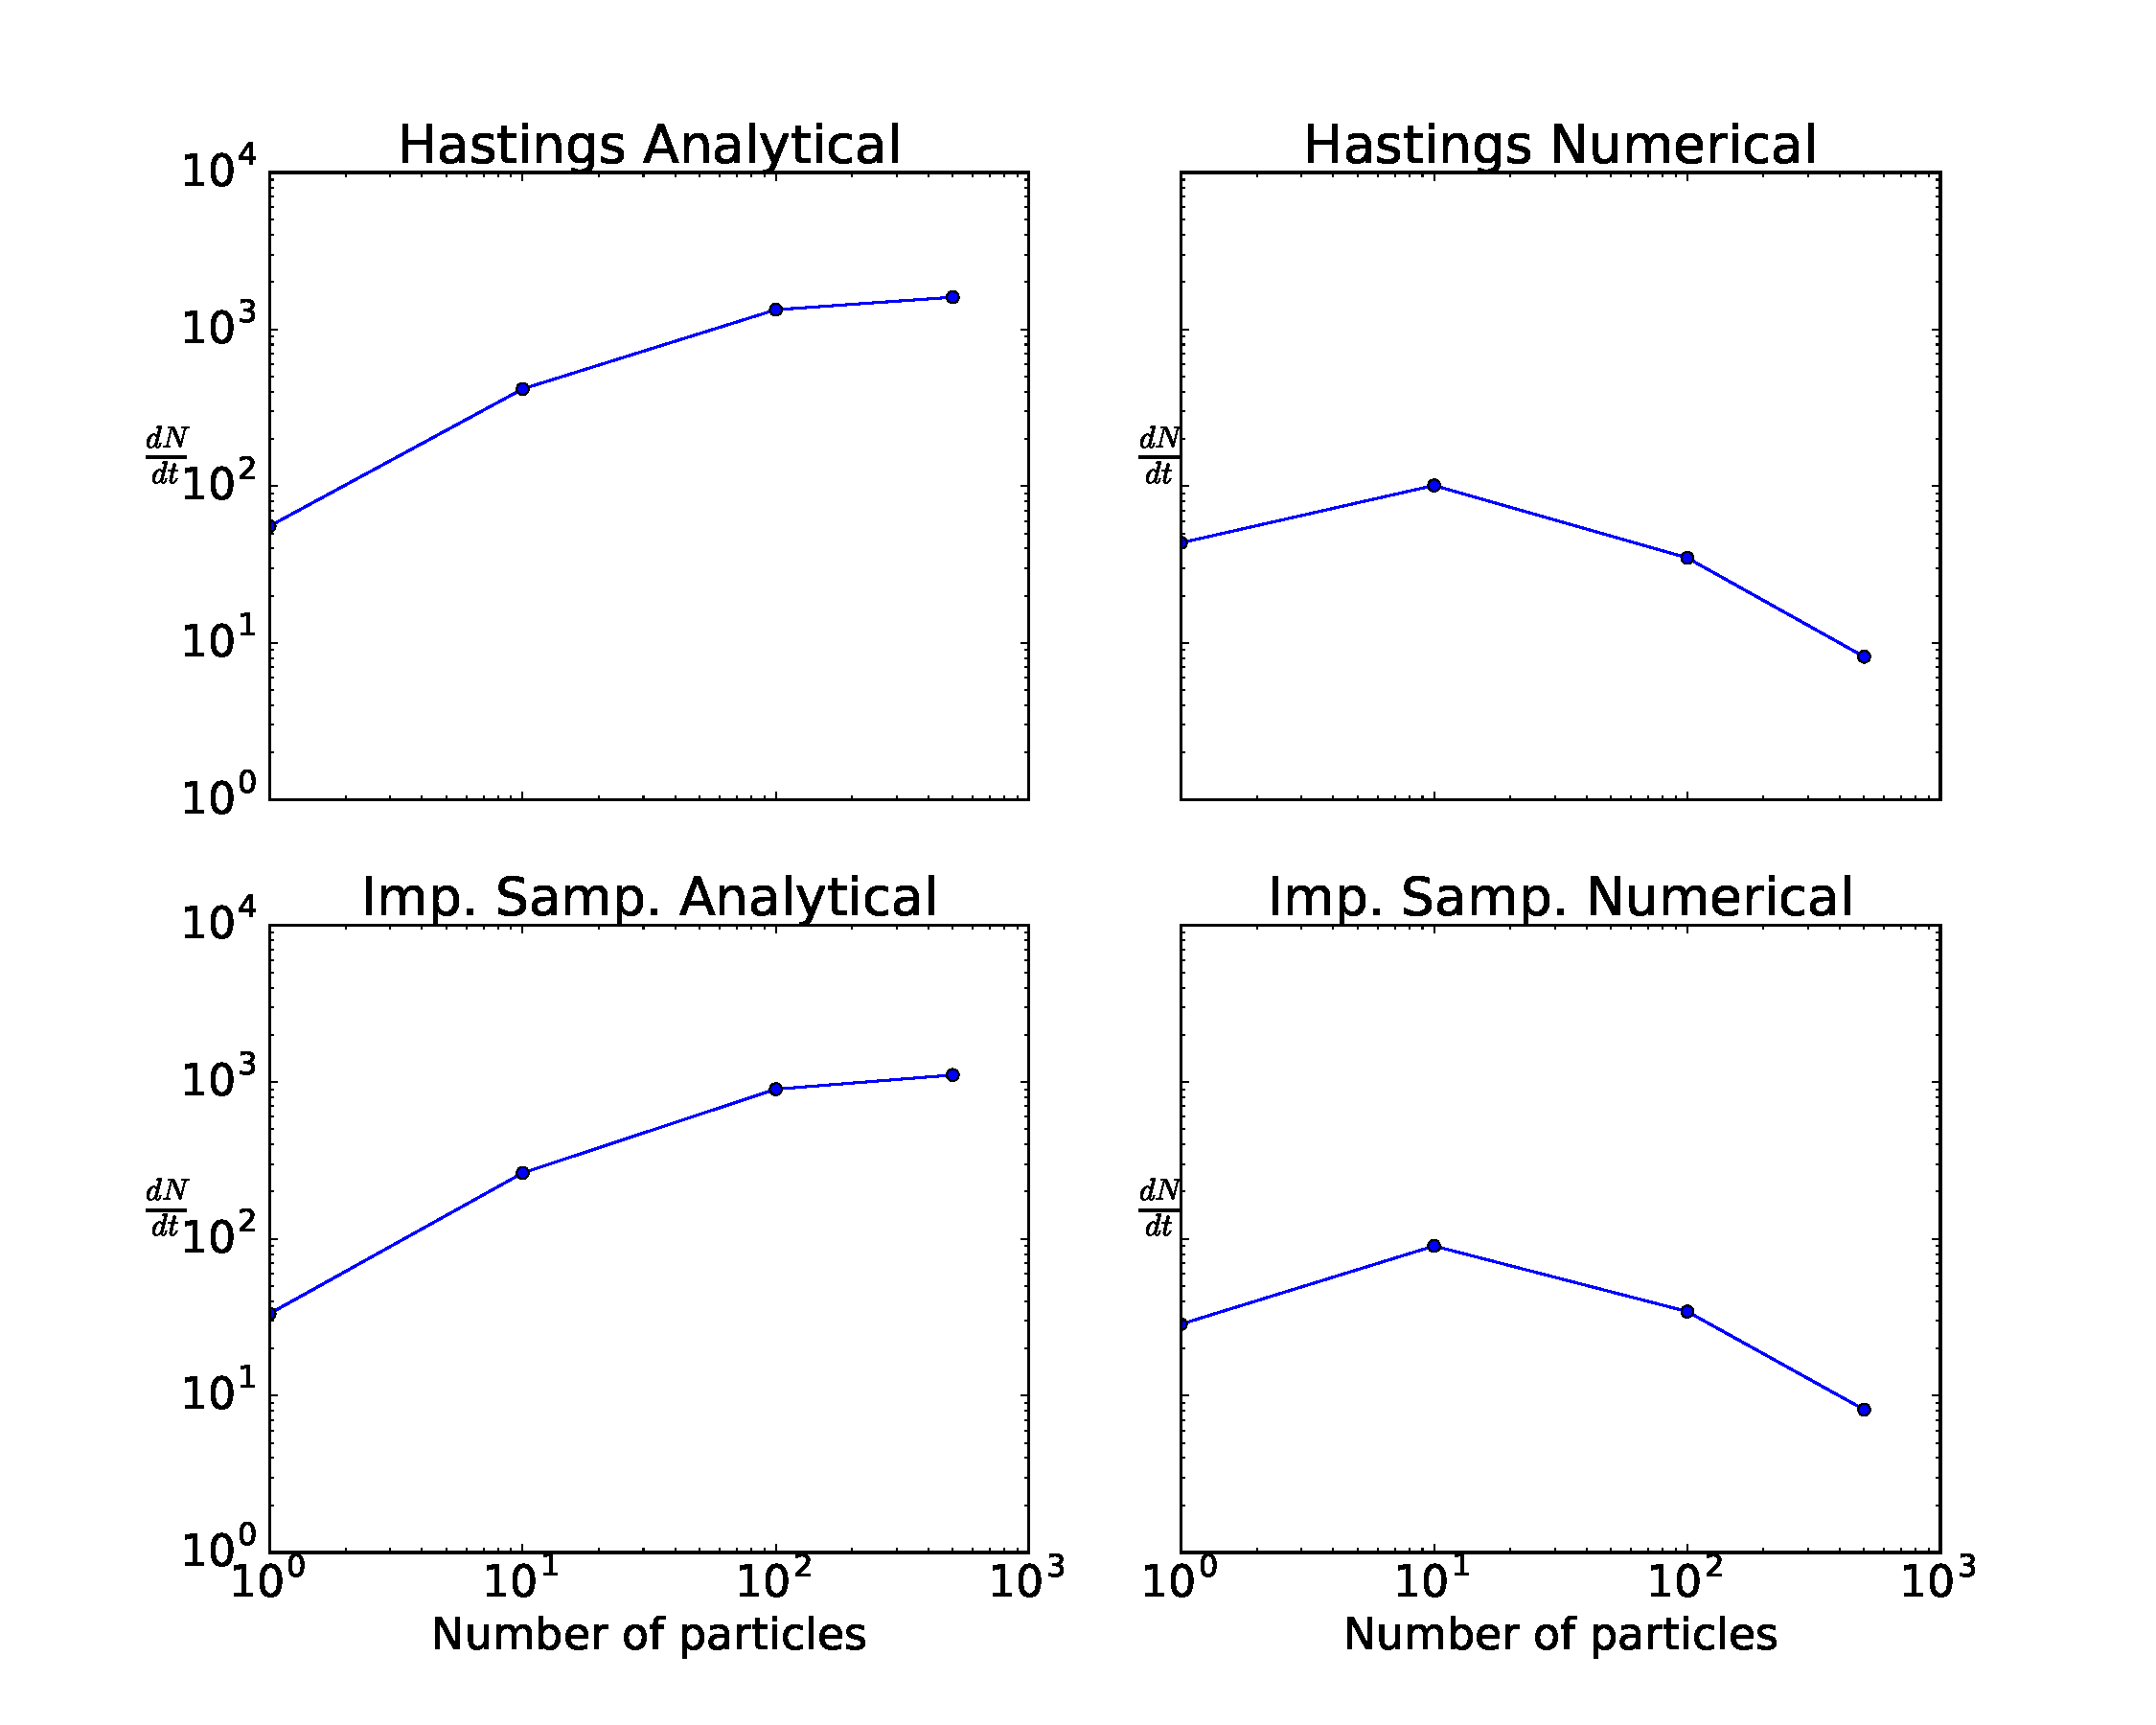
\includegraphics[scale=0.49]{graphs/Npart_time.pdf}
  }
    \caption{The x-axis is number of particles and y-axis are number of particles per time/step %
	     unit. The lower the graph goes, the more time per particle the program spends. %
	     This shows that the numerical Laplacians loses effectiveness as the number of %
	     particles grows, as for the analytical solutions the methods seem to converge %
	     toward a top.%
	     }
    
  \end{figure}
  For lower number of particles the time spent on operations other than calculating the energies
  is high. By increasing the number of particles the code spend more time calculating the
  laplacian and the graph seem to converge to a number around 1000 particles per unit
  step. With the numerical calculation of the Laplacian, the effectiveness of the computation
  decreases steeply as number of particles increases.
  
  \subsubsection{Interacting Hamiltonian}
  I could not find the error that was causing the interacting model to give bad results.
  There is an error increasing with number of particles, and it seems to have a linear
  correlation with the number of particles. It is also unstable, where it suddenly
  becomes NAN or similar. I have even compared my program with others and I can not find the error
  unfortunatly. I am hoping to get it fixed, but not in time for this report.
  \begin{figure}[h!]
    \centering
    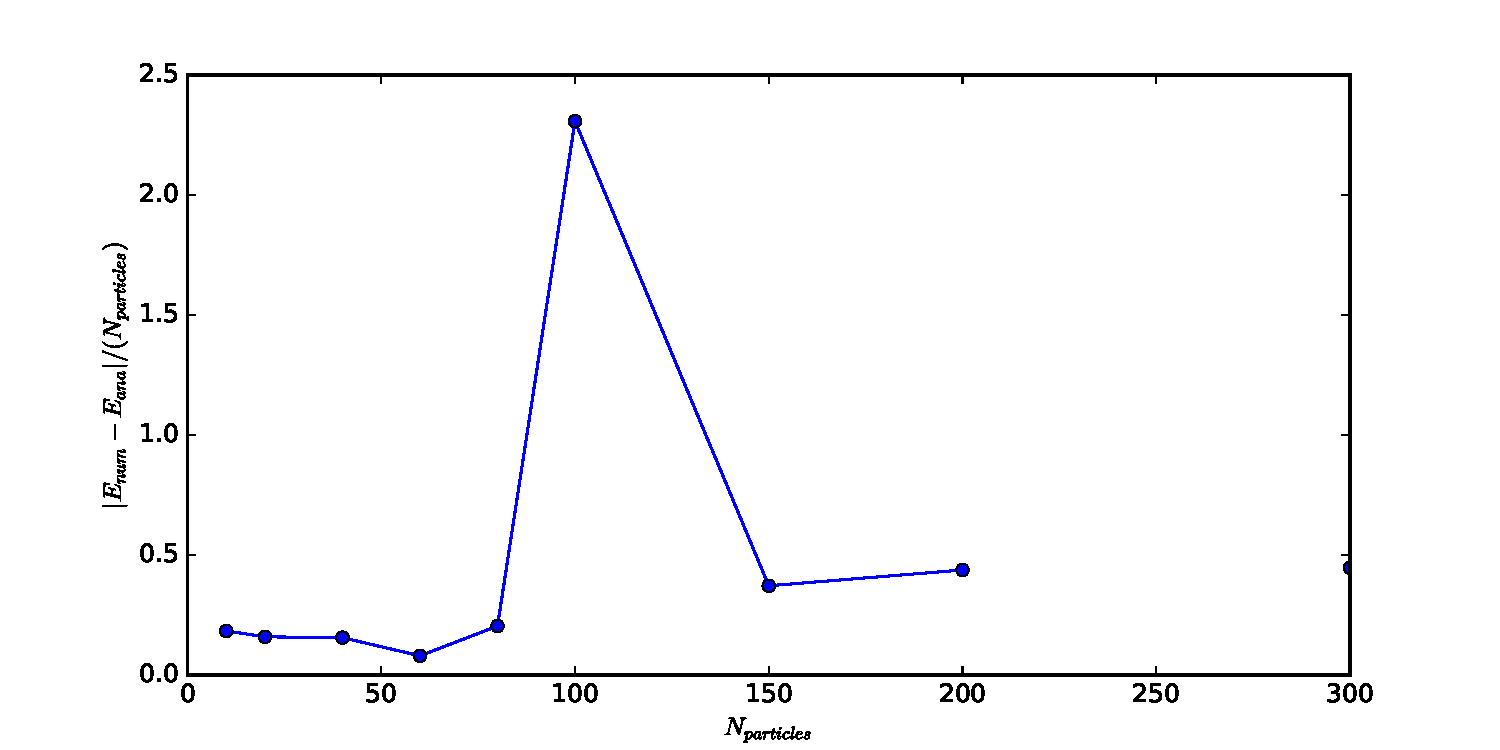
\includegraphics[scale=0.6]{graphs/errorana.pdf}
    \caption{Plotted on the y-axis is the mean energy difference between analytical and numerical %
      calculation per total number of particles. There seem to be a linear corerlation between %
      error with the the exceptions of some unstable parts. This might suggest that the error %
      might come from the movement of particles or in one of the single loops.}
  \end{figure}

  \newpage
  \subsubsection{Blocking}
  These are the results from a run of 500 particles with Importance Sampling since I do not have
  any interacting data to use.
  \begin{figure}[h!]
    \centering
    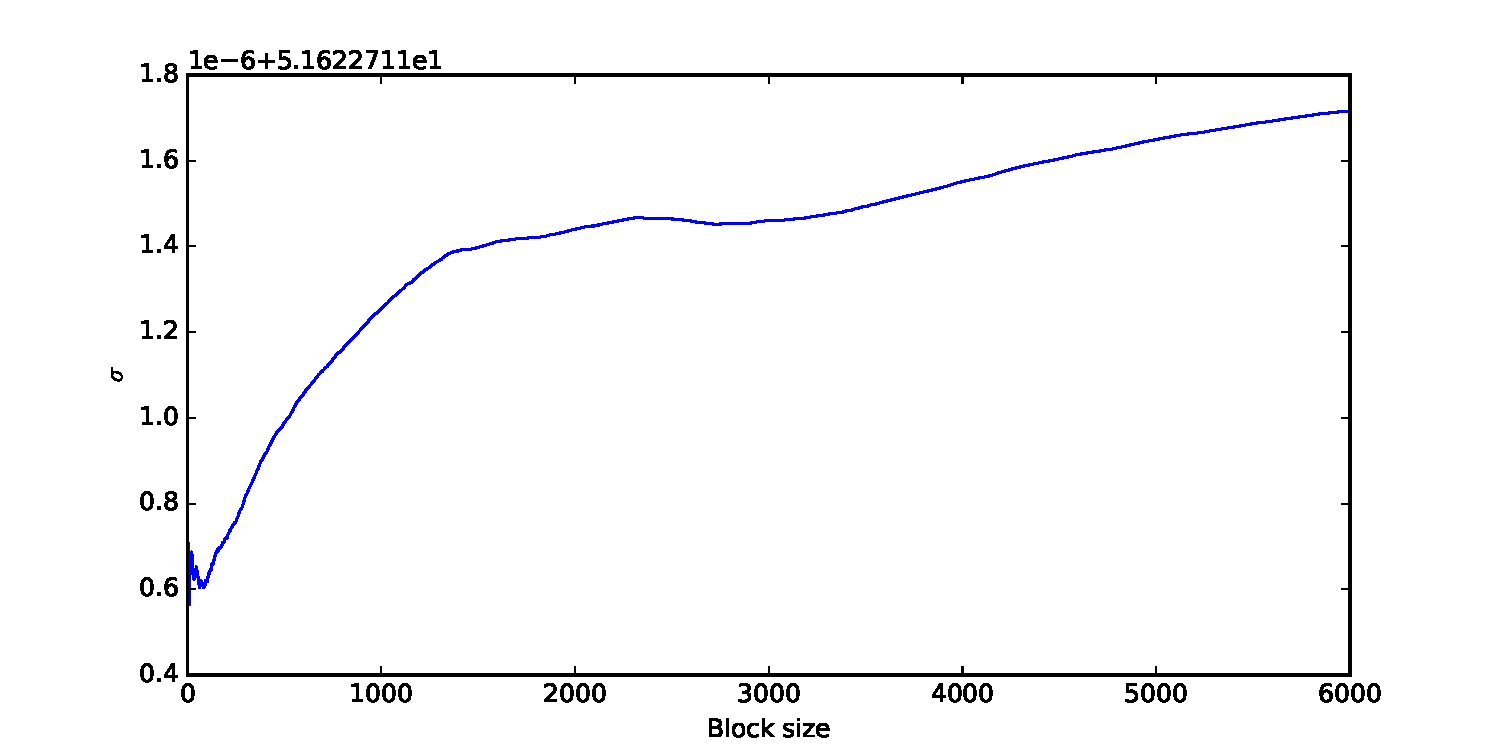
\includegraphics[scale=0.6]{graphs/block.pdf}
    \caption{500 particles and 3 dimensions, $10^5$ Monte Carlo cycles, $\alpha =0.5$%
     There is a very low variance due to high precision when calculating this system which %
      makes it harder to see the effect of blocking even though we can see the right shape. %
    the STD varies with $1\text{E}-6$.}
  \end{figure}
 
  \newpage
  \subsubsection{Particle distribution}
  \begin{figure}[h!]
    \centering
    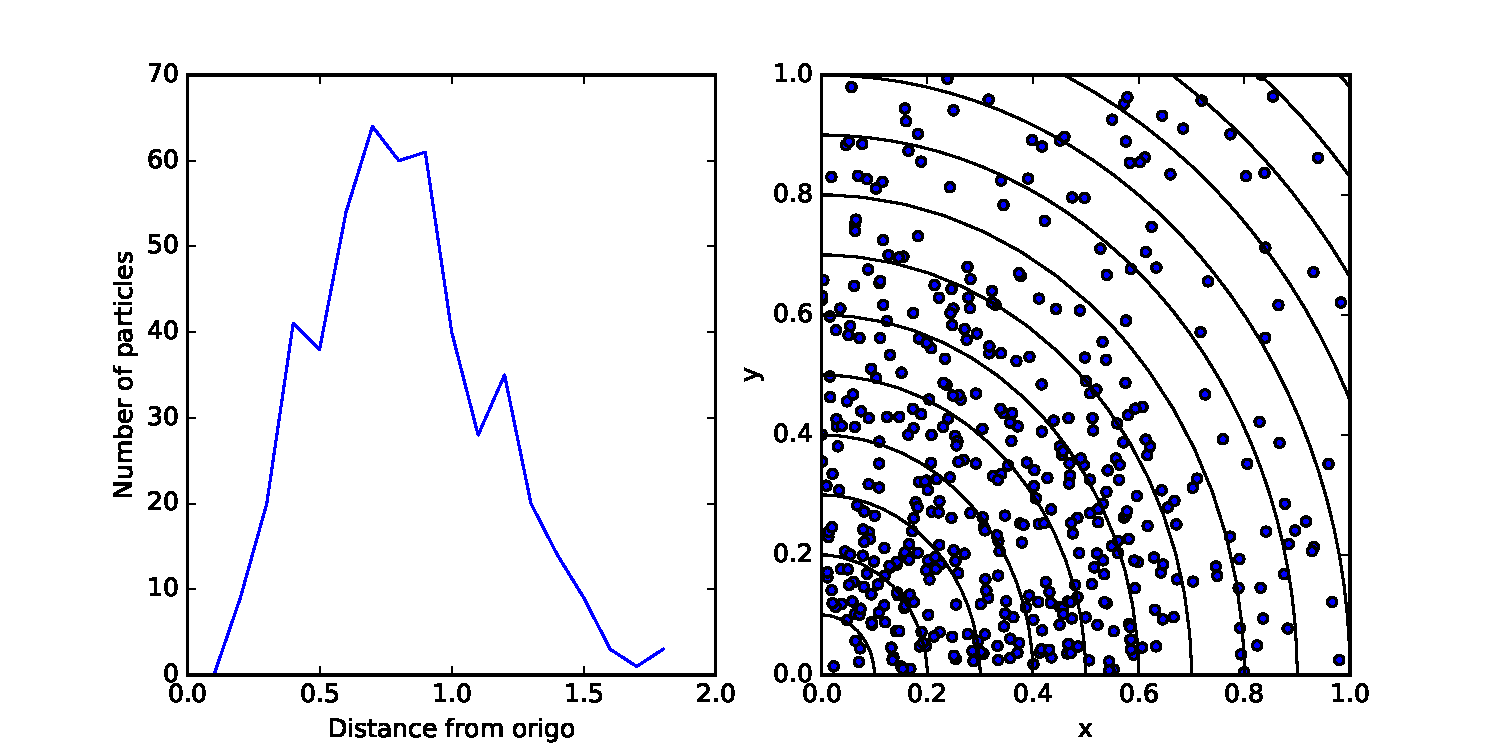
\includegraphics[scale=0.6]{graphs/dist.pdf}
    \caption{To the left is the distribution of particles after 8000 cycles %
      where we see a tendency to move towards 0.75. On the right side is a cross section %
      of the particles shown in the xy-plane, where the lines are the shells %
      chosen when counting the distribution.}
  \end{figure}

  \section{Conclusion}
  For the non-interacting system the VMC gave the exact results we would expect, and comparing
  the analytical solutions to the numerical showed little difference in result, but a significant
  increase in efficiency. Giving such low variance making it unnessecary to utilize blocking for 
  this system.
  The interacting system gave a high level of resistance when trying to compute the energies, only
  reaching a small amount of accuracy for 10 particles with the numerical solution.
  Furterhmore I hope to find the missing puzzle piece to get it up and running as fast as possible.
  
  \newpage
  \appendix
  \newpage
\section{Tables}
\subsection{Brute force Metropolis algorithm}
All runs are with with $10^5$ cycles and step length
of 1.7.
%\subsubsection{Analytical 1D}
%\begin{table}[h!]
\centering 
\begin{tabular}{|l|l|l|l|l|}
\hline 
N particles & $<E>$ & Variance & Accepted & Time [s]\\ 
 \hline 
1 & 5.000000e-01 & 0.000000e+00 & 0.553895 & 0.018 \\ \hline 
10 & 5.000000e+00 & 0.000000e+00 & 0.548784 & 0.024 \\ \hline 
100 & 5.000000e+01 & 0.000000e+00 & 0.550417 & 0.075 \\ \hline 
500 & 2.500000e+02 & 0.000000e+00 & 0.550962 & 0.312 \\ \hline 
\end{tabular}
\label{tab:ha1} 
\end{table} 

\subsubsection{Analytical 2D}
\begin{table}[h!]
\begin{tabular}{|l|l|l|l|l|}
\hline 
N particles & $<E>$ & Variance & Accepted & Time [ms]\\ 
 \hline 
1 & 1.000000e+00 & 0.000000e+00 & 0.968367 & 470 \\ \hline 
10 & 1.000000e+01 & 0.000000e+00 & 0.967963 & 711 \\ \hline 
100 & 1.000000e+02 & 0.000000e+00 & 0.968089 & 2808 \\ \hline 
500 & 5.000000e+02 & 0.000000e+00 & 0.968799 & 12433 \\ \hline 
\end{tabular}
\label{h:a2} 
\end{table}

\subsubsection{Analytical 3D}
\begin{tabular}{|l|l|l|l|l|}
\hline 
\multicolumn{5}{|c|}{Analytical}\\ 
\hline 
N particles & $<E>$ & Variance & Accepted & Time [ms]\\ 
 \hline 
1 & 1.500000e+00 & 0.000000e+00 & 0.968941 & 484 \\ 
\hline10 & 1.500000e+01 & 0.000000e+00 & 0.967473 & 792 \\ 
\hline100 & 1.500000e+02 & 0.000000e+00 & 0.968197 & 3623 \\ 
\hline500 & 7.500000e+02 & 0.000000e+00 & 0.969128 & 16629 \\ 
\hline\end{tabular}
%\subsubsection{Numerical 1D}
%\begin{table}[h!]
\centering 
\begin{tabular}{|l|l|l|l|l|}
\hline 
N particles & $<E>$ & Variance & Accepted & Time [s]\\ 
 \hline 
1 & 5.000000e-01 & -9.436896e-16 & 0.550639 & 0.023 \\ \hline 
10 & 5.000000e+00 & -5.115908e-13 & 0.548139 & 0.099 \\ \hline 
100 & 5.000000e+01 & 3.092282e-11 & 0.551551 & 2.868 \\ \hline 
500 & 2.500000e+02 & 3.419700e-10 & 0.550273 & 61.191 \\ \hline 
\end{tabular}
\caption{%
	  Benchmark of the brute force Metropolis method with %
	  numerical calculation of the Laplacian. Using $10^5$ %
	  cycles and a step length of 1.7.%
	}
\label{tab:hn1} 
\end{table} 

\newpage
\subsubsection{Numerical 2D}
\begin{tabular}{|l|l|l|l|l|}
\hline 
\multicolumn{5}{|c|}{Numerical 2D}\\ 
\hline 
N particles & $<E>$ & Variance & Accepted & Time [ms]\\ 
 \hline 
1 & 9.999999e-01 & 6.494805e-14 & 0.968163 & 751 \\ \hline 
10 & 9.999999e+00 & 1.747935e-12 & 0.968789 & 5478 \\ \hline 
100 & 9.999999e+01 & 1.618901e-10 & 0.968061 & 235928 \\ \hline 
500 & 5.000000e+02 & 2.732850e-08 & 0.969589 & 5144598 \\ \hline 
\label{h:n2} 
\end{tabular}
\subsubsection{Numerical 3D}
\begin{tabular}{|l|l|l|l|l|}
\hline 
\multicolumn{5}{|c|}{Numerical}\\ 
\hline 
N particles & $<E>$ & Variance & Accepted & Time [ms]\\ 
 \hline 
1 & 1.500000e+00 & 1.509903e-14 & 0.968088 & 917 \\ 
\hline100 & 1.500000e+02 & 2.619345e-10 & 0.967844 & 415179 \\ 
\hline100 & 1.500000e+02 & -7.275958e-11 & 0.968416 & 413230 \\ 
\hline500 & 7.499999e+02 & -3.352761e-08 & 0.969971 & 9641421 \\ 
\hline\end{tabular}
\newpage
\subsection{Metropolis algorithm with Importance sampling}
All runs are with with $10^5$ cycles and step length
of 0.05.
%\subsubsection{Analytical 1D}
%\begin{table}[h!]
\begin{tabular}{|l|l|l|l|l|}
\hline 
N particles & $<E>$ & Variance & Accepted & Time [s]\\ 
 \hline 
1 & 5.000000e-01 & 0.000000e+00 & 0.998522 & 0.03 \\ \hline 
10 & 5.000000e+00 & 0.000000e+00 & 0.998700 & 0.038 \\ \hline 
100 & 5.000000e+01 & 0.000000e+00 & 0.998644 & 0.111 \\ \hline 
500 & 2.500000e+02 & 0.000000e+00 & 0.998922 & 0.451 \\ \hline 
\end{tabular}
\label{tab:ia1} 
\end{table} 

\subsubsection{Analytical 2D}
\begin{table}[h!]
\begin{tabular}{|l|l|l|l|l|}
\hline 
N particles & $<E>$ & Variance & Accepted & Time [s]\\ 
 \hline 
1 & 1.000000e+00 & 0.000000e+00 & 0.998744 & 0.03 \\ \hline 
10 & 1.000000e+01 & 0.000000e+00 & 0.998644 & 0.044 \\ \hline 
100 & 1.000000e+02 & 0.000000e+00 & 0.998689 & 0.181 \\ \hline 
500 & 5.000000e+02 & 0.000000e+00 & 0.998800 & 0.817 \\ \hline 
\end{tabular}
\label{tab:ia2} 
\end{table} 

\subsubsection{Analytical 3D}
\begin{tabular}{|l|l|l|l|l|}
\hline 
\multicolumn{5}{|c|}{Analytical}\\ 
\hline 
N particles & $<E>$ & Variance & Accepted & Time [ms]\\ 
 \hline 
1 & 1.500000e+00 & 0.000000e+00 & 0.996373 & 780 \\ 
\hline10 & 1.500000e+01 & 0.000000e+00 & 0.996321 & 1198 \\ 
\hline100 & 1.500000e+02 & 0.000000e+00 & 0.996450 & 5396 \\ 
\hline500 & 7.500000e+02 & 0.000000e+00 & 0.996357 & 24110 \\ 
\hline\end{tabular}
%\subsubsection{Numerical 1D}
%\begin{table}[h!]
\begin{tabular}{|l|l|l|l|l|}
\hline 
N particles & $<E>$ & Variance & Accepted & Time [ms]\\ 
 \hline 
1 & 4.999999e-01 & 1.915135e-15 & 0.996353 & 839 \\ \hline 
10 & 4.999999e+00 & -2.351896e-12 & 0.996342 & 2724 \\ \hline 
100 & 4.999999e+01 & 3.310561e-10 & 0.996470 & 68701 \\ \hline 
500 & 2.500000e+02 & 5.456968e-10 & 0.996473 & 1410677 \\ \hline 
\end{tabular}
\label{i:n1} 
\end{table}

\subsubsection{Numerical 2D}
\begin{table}[h!]
\begin{tabular}{|l|l|l|l|l|}
\hline 
N particles & $<E>$ & Variance & Accepted & Time [s]\\ 
 \hline 
1 & 9.999999e-01 & 1.099121e-14 & 0.998756 & 0.041 \\ \hline 
10 & 9.999999e+00 & 6.963319e-13 & 0.998767 & 0.223 \\ \hline 
100 & 9.999999e+01 & 2.546585e-11 & 0.998711 & 10.117 \\ \hline 
500 & 4.999999e+02 & -5.587935e-09 & 0.998789 & 232.673 \\ \hline 
\end{tabular}
\label{tab:in2} 
\end{table} 

\subsubsection{Numerical 3D}
\begin{tabular}{|l|l|l|l|l|}
\hline 
\multicolumn{5}{|c|}{Numerical}\\ 
\hline 
N particles & $<E>$ & Variance & Accepted & Time [ms]\\ 
 \hline 
1 & 1.500000e+00 & 1.243450e-13 & 0.996377 & 1198 \\ 
\hline10 & 1.500000e+01 & 6.025402e-12 & 0.996434 & 9108 \\ 
\hline100 & 1.500000e+02 & 1.615263e-09 & 0.996397 & 429843 \\ 
\hline500 & 7.499999e+02 & -9.709038e-08 & 0.996334 & 9671595 \\ 
\hline\end{tabular}

  \bibliographystyle{unsrt}
  \bibliography{report}
\end{document}
